\chapter{Introduction}
\label{chapter:intro}

{\color{red} TODO: hyphenation}

{\color{red} TODO: spell check}

{\color{red} TODO: consistent tense}

{\color{red} TODO: acknowledgements for ALL scenes, images, Mitsuba, \dots}

Most people nowadays are familiar with \textit{projection}, the act of transferring images from film or computer memory onto screens in cinemas and classrooms. But while those screens are made specifically for being projected onto, this is not the case for other objects, for example building façades. The geometry and material properties of these objects deform projected images and change their appearance. This is why projecting them is not enough -- they first need to be edited (\textit{mapped}) in a way that their final appearance is what we expect. Projecting onto arbitrary objects in such a way is called \textit{projection mapping} and it is the main topic of this thesis.

\begin{figure}[ht]
    \centering
    \begin{subfigure}[b]{0.49\textwidth}
        \centering
        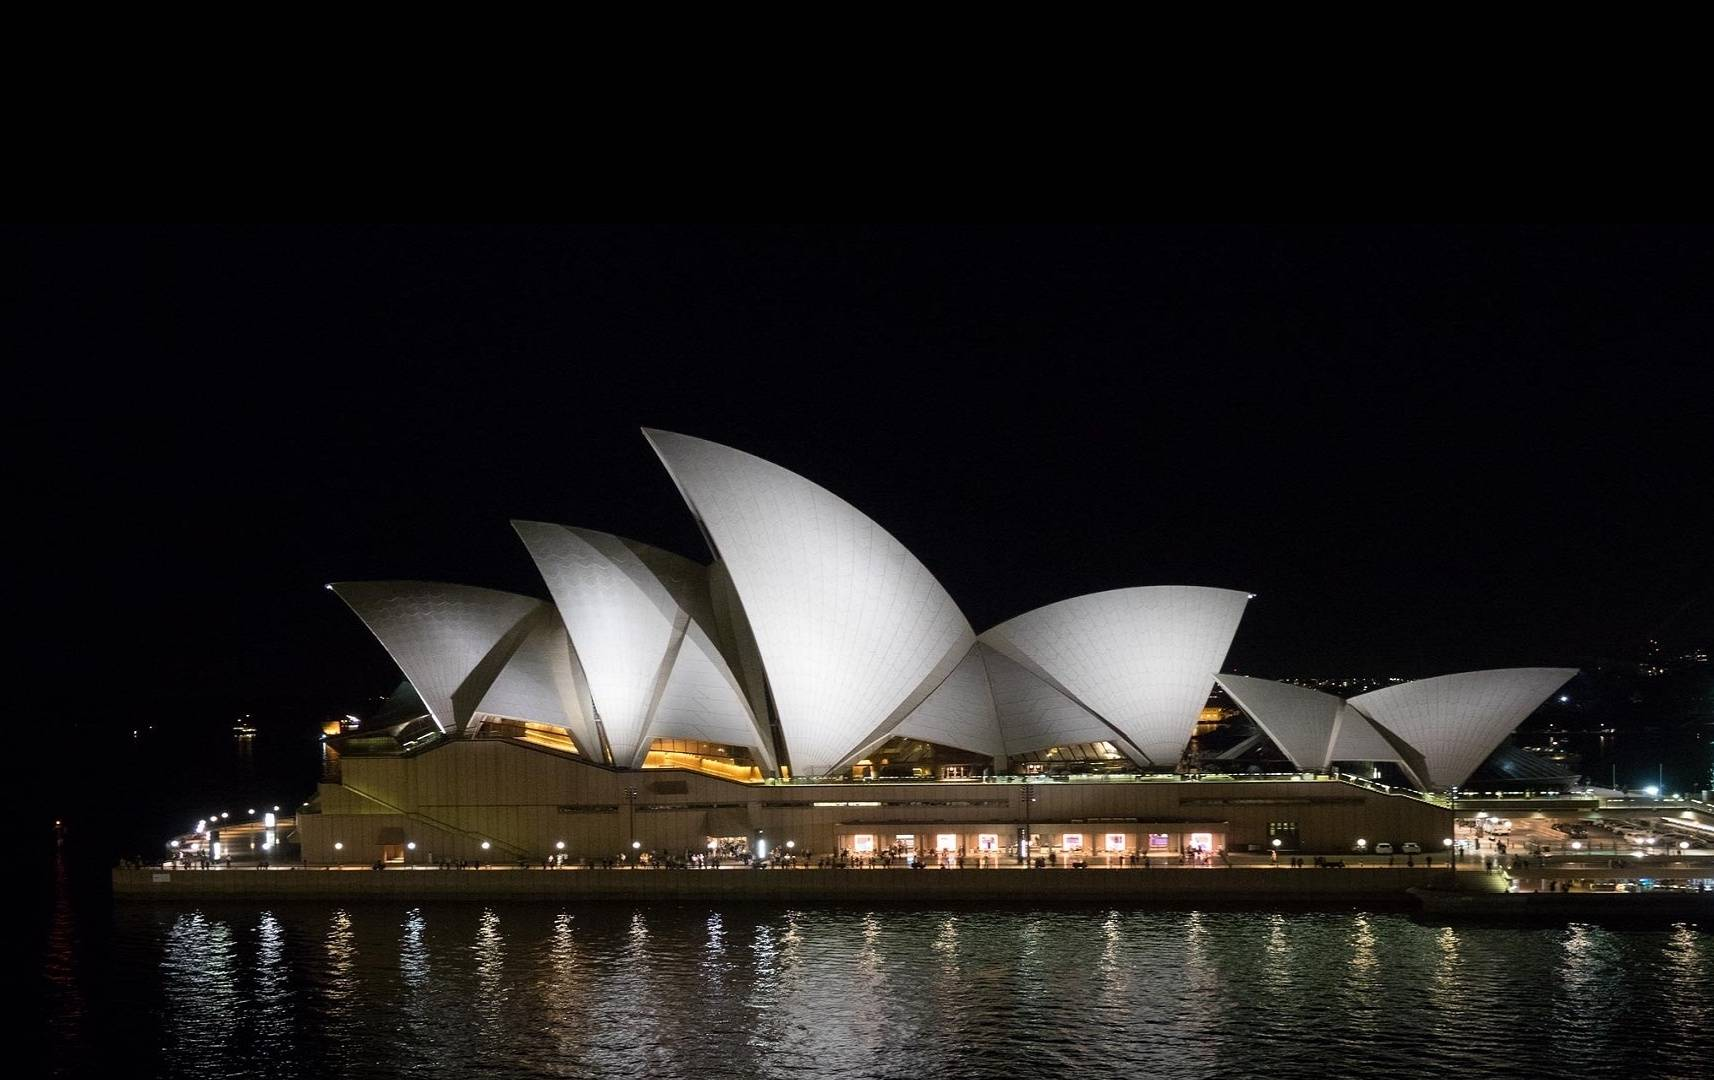
\includegraphics[width=\textwidth]{images/01-sydney_opera_house_night-edit.jpg}
        \caption{}
        %\label{}
    \end{subfigure}
    \hfill
    \begin{subfigure}[b]{0.49\textwidth}
        \centering
        \includegraphics[width=\textwidth]{images/01-sydney_opera_house_projection1.jpg}
        \caption{Source: \citet{ImageProjectionMappingExampleSydney}}
        %\label{}
    \end{subfigure}
    \caption{The Sydney Opera House with (b) and without (a) projection mapping.}
    \label{fig:intro_example_sydney}
\end{figure}

One of the first uses of projection mapping (also sometimes called \textit{video mapping} or \textit{spatial augmented reality}) was in the character of Madame Leota in The Haunted Mansion Disneyland ride which opened in 1969. There, a video of a human face was projected onto a static head (see fig. \ref{fig:intro_example_leota}). Nowadays, projection mapping has become widespread. It is used to augment reality by artists from all over the world in galleries, museums and outdoor spaces. One prominent example is projection mapping on buildings (see fig. \ref{fig:intro_example_sydney}) which is done in cities during festivals and on other special occasions.

\begin{figure}[ht]
    \centering
    \begin{subfigure}{0.6\textwidth}
        \centering
        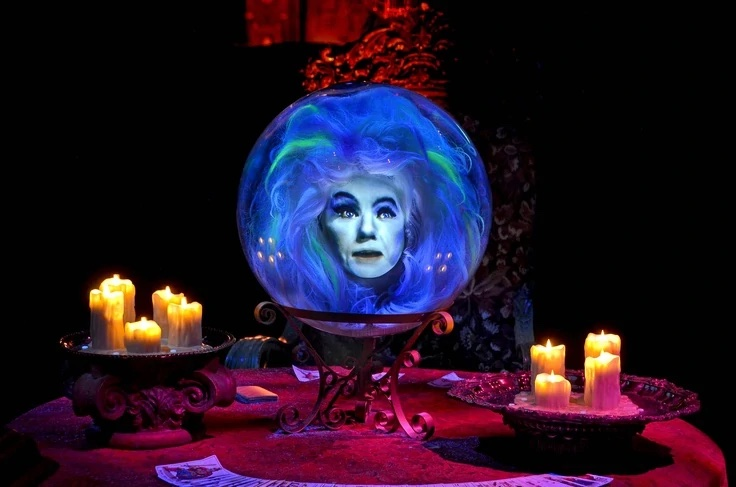
\includegraphics[width=\textwidth]{images/01-Leota.jpg}
        \caption{}
        \label{fig:intro_example_leota-full}
    \end{subfigure}
    \hfill
    \begin{subfigure}{0.39\textwidth}
        \centering
        \begin{subfigure}{\textwidth}
            \centering
            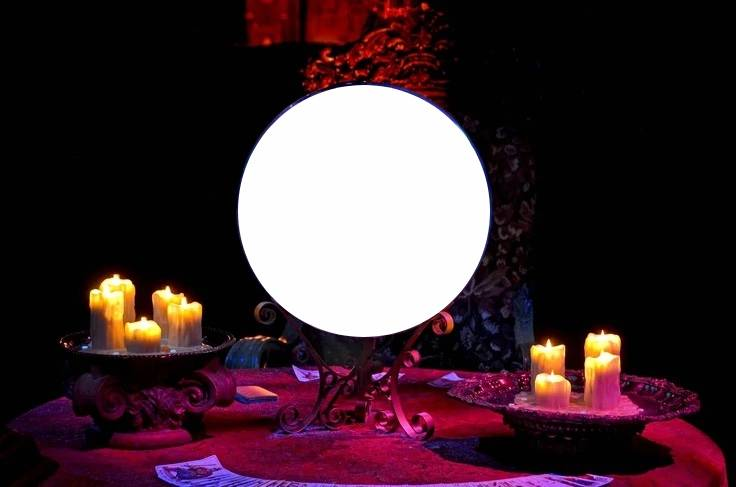
\includegraphics[width=\textwidth]{images/01-Leota-no_head.jpg}
            \caption{}
            \label{fig:intro_example_leota-scene}
        \end{subfigure}
        
        \begin{subfigure}{\textwidth}
            \centering
            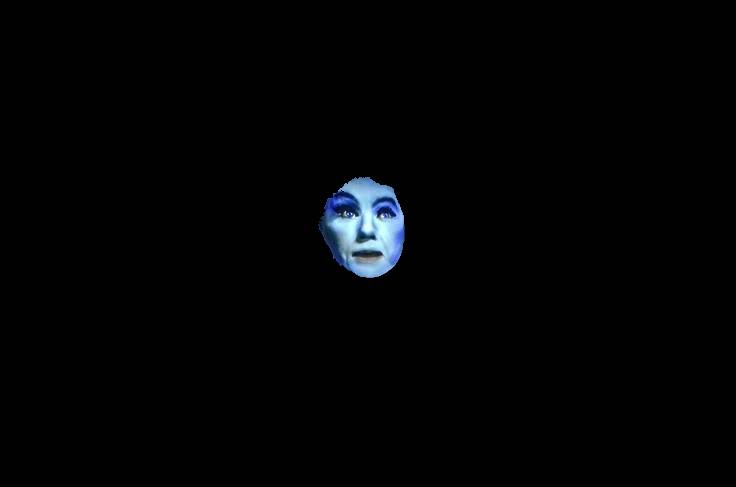
\includegraphics[width=\textwidth]{images/01-Leota-only_head.jpg}
            \caption{}
            \label{fig:intro_example_leota-head}
        \end{subfigure}
    \end{subfigure}
    \caption{The character of Madame Leota in Disneyland's Haunted Mansion ride is one of the earliest examples of projection mapping. A video of her face is projected onto a neutrally colored static form inside a glass ball to give an illusion that the form speaks (\citet{MadameLeota}). Included is our simplified decomposition of the scene (\ref{fig:intro_example_leota-full}) into background (\ref{fig:intro_example_leota-scene}) and projection image (\ref{fig:intro_example_leota-head})}
    \label{fig:intro_example_leota}
\end{figure}

Let us now briefly describe what projection mapping entails and which of its problems we aim to address in this thesis.

\section{Problem Setting}
\label{section:intro-problem_setting}

Simply put, projection mapping is projecting onto surfaces that are not primarily intended for projection and often have complex texture or geometry. In this thesis, we formulate the projection mapping problem as follows:

\begin{enumerate}
    \item We begin with a scene, for example fig. \ref{fig:intro_example_leota-scene}
    \item We choose what we would want it to look like after projection (i.e. the \textit{desired appearance}), for example fig. \ref{fig:intro_example_leota-full}
    \item The task is to create a \textit{compensated projection image} that will look like our desired appearance when projected onto our scene, for example fig. \ref{fig:intro_example_leota-head}
    \item We project the compensated image
\end{enumerate}

There is a wide body of research focusing on creating such compensated images automatically given a scene and a desired appearance. In one of the earliest papers of the field, \citet{Grossberg2004} project a series of special calibration images onto a scene and capture their appearance using a camera. Using these \textit{camera images}, they are able to estimate how each pixel of the projection influences the appearance of that particular scene. Once this calibration is ready, they are able to quickly compute compensation images on the fly and only project the compensations (see fig. \ref{fig:intro_grossberg} for an example). The combination of a projector and a camera is common in projection mapping and such systems are called \textit{projector-camera systems} (see fig. \ref{fig:intro_procam}).

\begin{figure}[ht]
    \centering    
    \begin{subfigure}{0.8\textwidth}
        \centering
        \begin{subfigure}{0.3\textwidth}
            \centering
            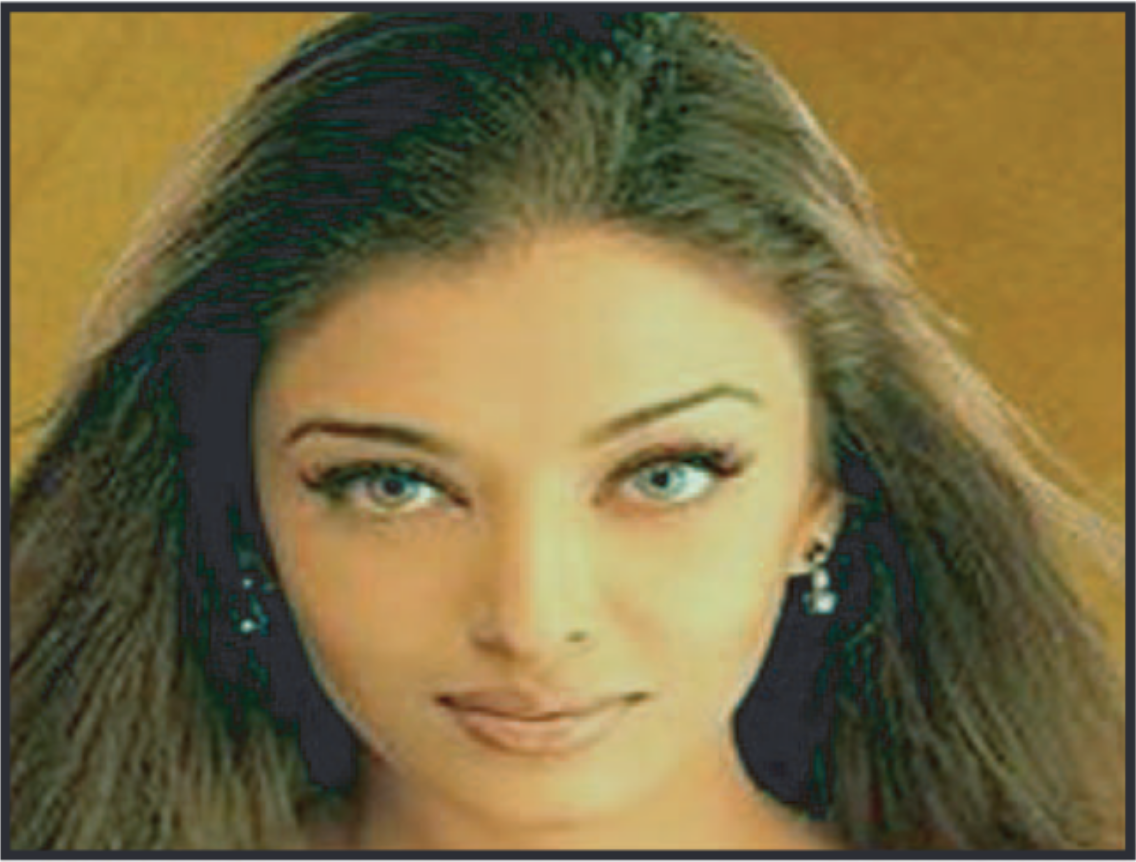
\includegraphics[width=\textwidth]{images/01-desired_appearance.png}
            \caption{Desired appearance}
            \label{fig:intro_grossberg-desired_appearance}
        \end{subfigure}
        \hfill
        \begin{subfigure}{0.3\textwidth}
            \centering
            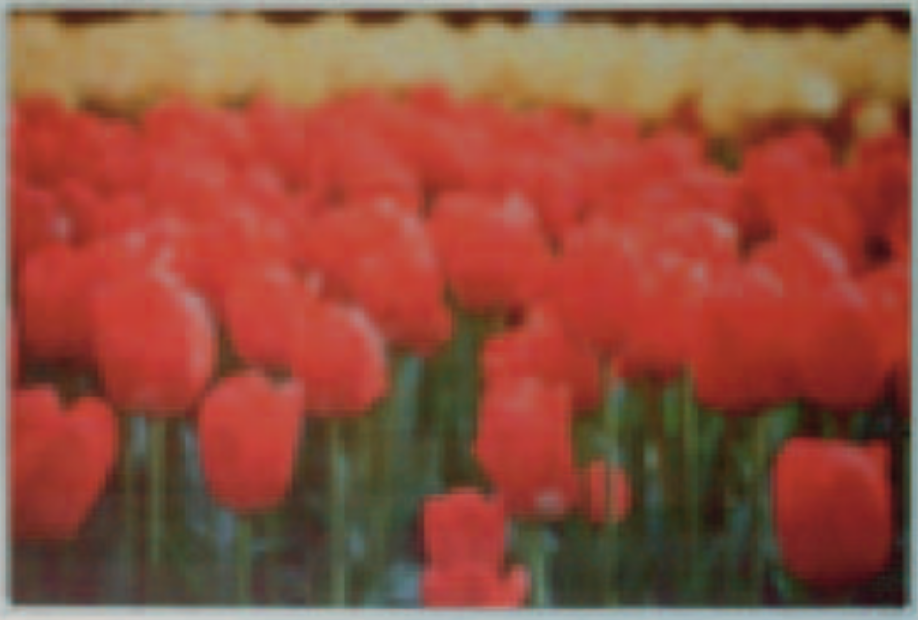
\includegraphics[width=\textwidth]{images/01-background.png}
            \caption{Background}
            \label{fig:intro_grossberg-background}
        \end{subfigure}
        \hfill
        \begin{subfigure}{0.3\textwidth}
            \centering
            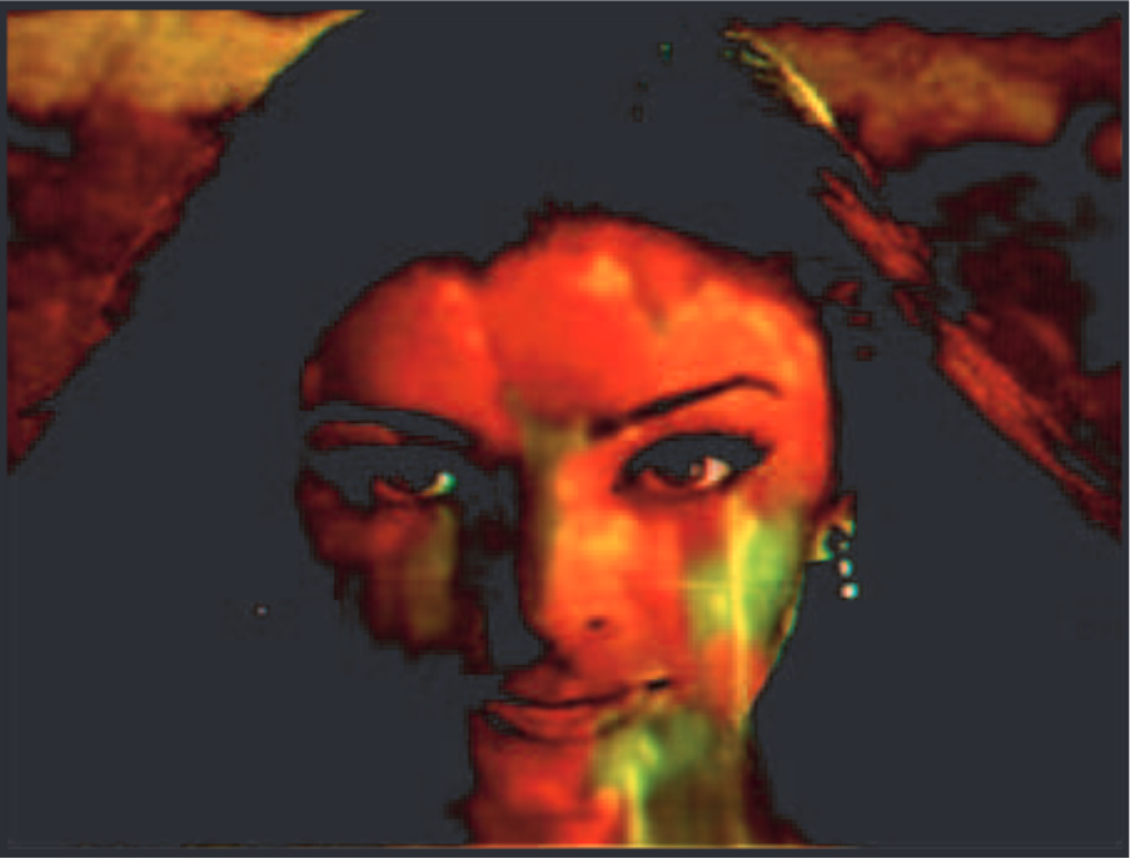
\includegraphics[width=\textwidth]{images/01-uncompensated.png}
            \caption{\ref{fig:intro_grossberg-desired_appearance} projected onto \ref{fig:intro_grossberg-background}}
            \label{fig:intro_grossberg-uncompensated}
        \end{subfigure}
        
        \begin{subfigure}{0.3\textwidth}
            \centering
            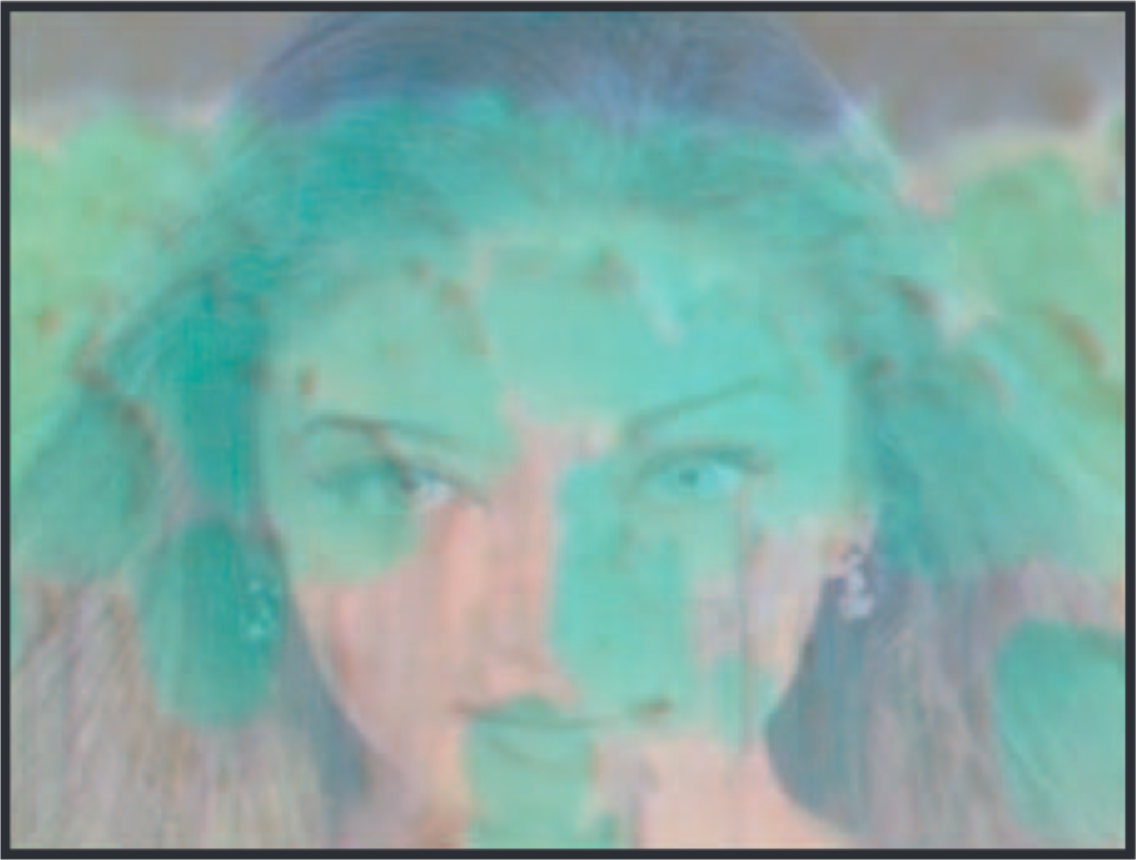
\includegraphics[width=\textwidth]{images/01-compensation_image.png}
            \caption{Compensated projection image}
            \label{fig:intro_grossberg-compensation}
        \end{subfigure}
        \hfill
        \begin{subfigure}{0.3\textwidth}
            \centering
            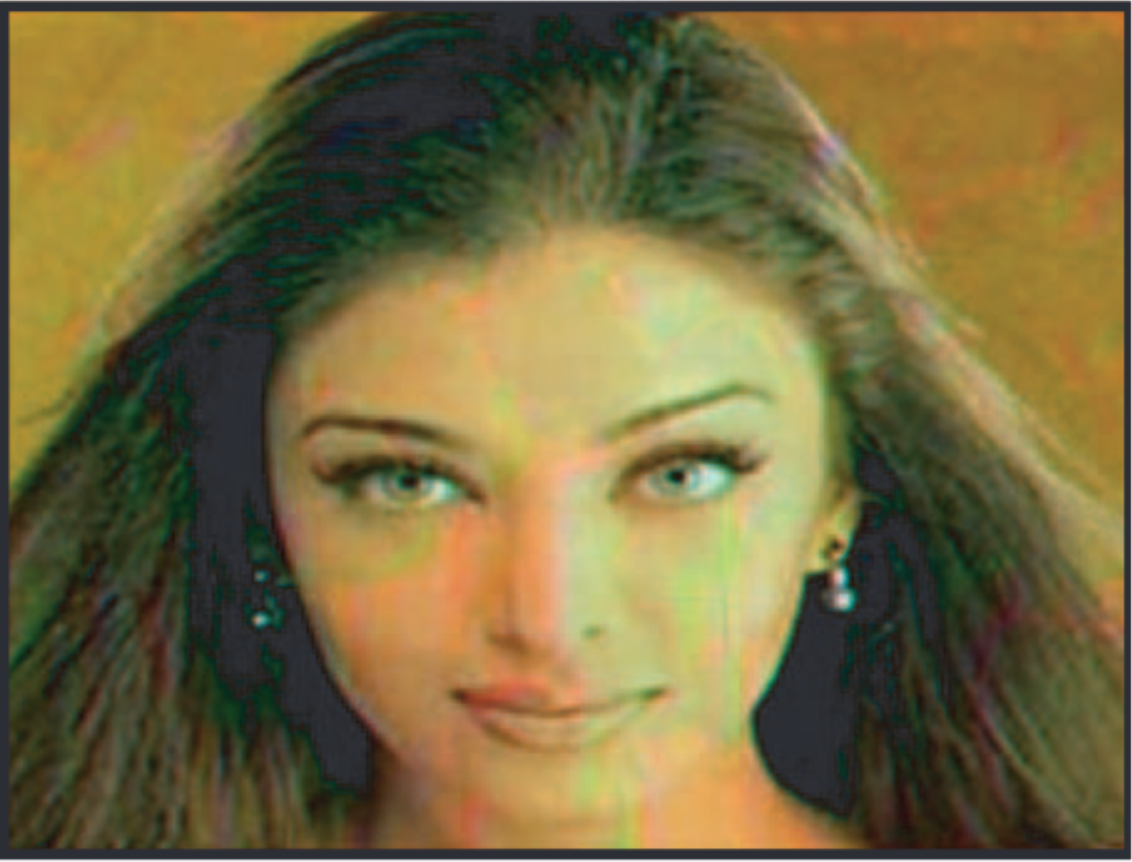
\includegraphics[width=\textwidth]{images/01-new_appearance.png}
            \caption{\ref{fig:intro_grossberg-compensation} projected onto \ref{fig:intro_grossberg-background}}
            \label{fig:intro_grossberg-new_appearance}
        \end{subfigure}
    \end{subfigure}
    \caption{Automatic projection mapping as presented in \citet{Grossberg2004}}
    \label{fig:intro_grossberg}
\end{figure}

\begin{figure}[ht]
    \centering
    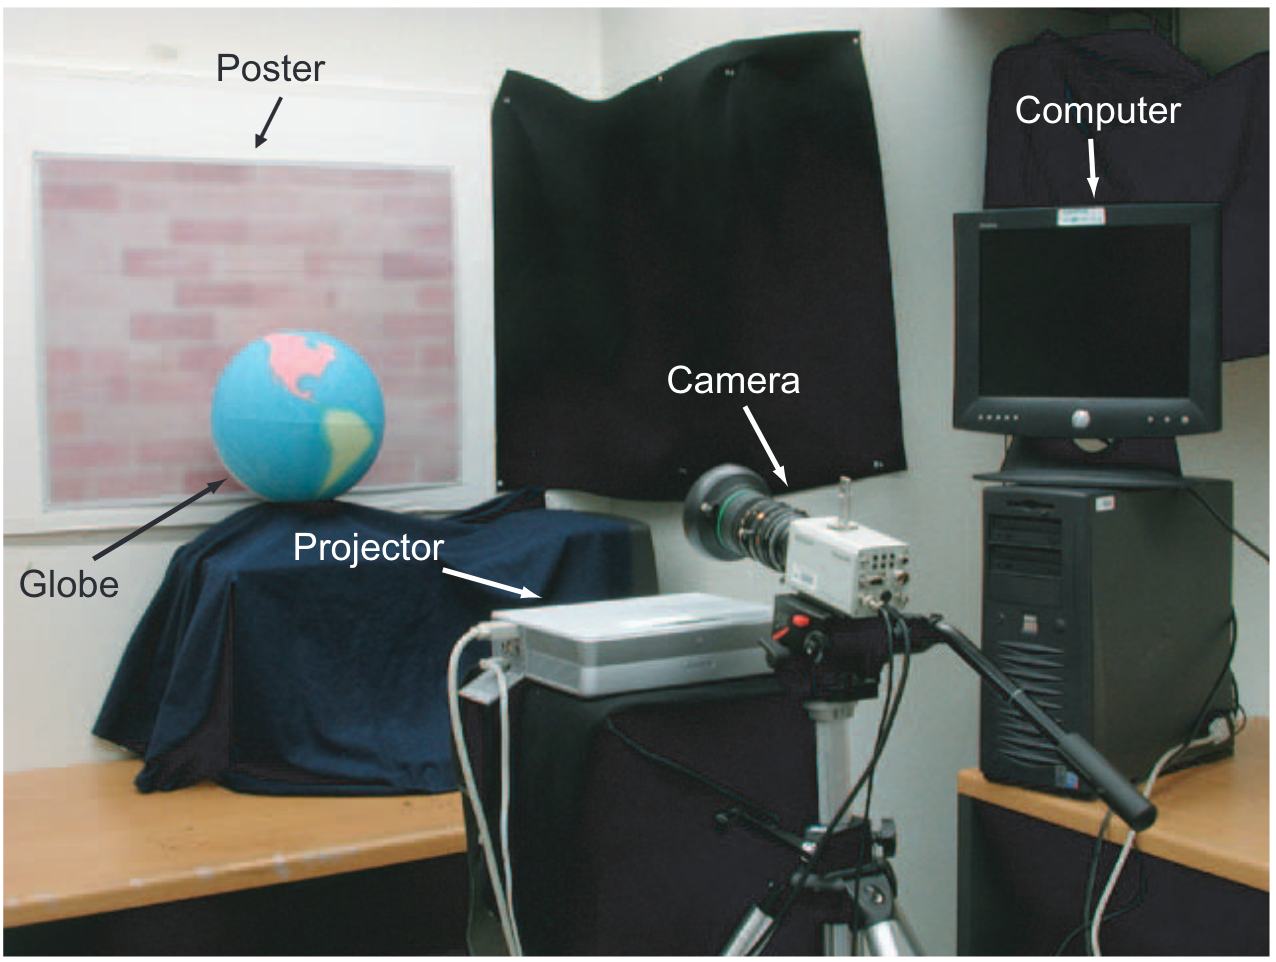
\includegraphics[width=0.6\textwidth]{images/01-procam.png}
    \caption{Projector-camera system from \citet{Grossberg2004}}
    \label{fig:intro_procam}
\end{figure}

Since then, there have been many advances in the field, the summary of which can be found in a state-of-the-art report by \citet{Grundhofer2018}. The latest projector-camera systems are able to calibrate themselves automatically after they are placed in a scene, re-calibrate when scene illumination changes, or when objects in the scene are transformed, both rigidly (i.e. without deformation) and non-rigidly. Some can do this in real time. Because of the sheer complexity of general projection mapping, however, no single method can do all these things at once. For example, methods that handle non-rigid transformations will often rely on object tracking which requires the object to have markers on it. Such methods might also break when illumination changes significantly.

There is, however, one fundamental characteristic that all current projection mapping methods share. When computing the compensated projection image, they match the camera image with the desired appearance pixel by pixel. Explicitly, their goal is the following:

\begin{equation}
    \label{eq:projection_mapping-per_pixel}
    \min_p \sum_{i=1}^{m \cdot n} || x(p)_{(i)} - y_{(i)} ||
\end{equation}

where \(p\) is the projector image, \(x(p) \in \mathbb{R}^{m \times n}\) is the camera image when \(p\) is projected, \(y\) is the desired appearance and \((i)\) selects the \(i\)-th pixel of an image. Note that \(x\) is determined by the projector and the scene.

This approach is limited by projector hardware. Every projector has finite brightness which means that pixels of the camera image cannot be made arbitrarily bright. In scenes with external illumination, it is also impossible to make pixels of the camera image arbitrarily dark since projectors can only add light and not subtract it. In the notation introduced above this means that for any projector image \(p\), we have

\begin{equation}
    \label{eq:projection_mapping-limitations}
    \forall i:\; 0 \leq x(p)_{(i)} \leq c_{(i)}
\end{equation}

where \(c\) is a constant vector that depends on the projector and the scene.

For every projector and scene, we can therefore find an image \(y\) whose pixels are too dark or too bright such that they cannot be mapped using the recipe in eq. \ref{eq:projection_mapping-per_pixel}:

\begin{equation}
    \label{eq:projection_mapping-hard_image}
    \exists i:\; y_{(i)} < 0 \lor y_{(i)} > c_{(i)}
\end{equation}

See fig. \ref{fig:intro_pixels_vs_stats} for examples.

\begin{figure}[ht]
    \centering    
    \begin{subfigure}{\textwidth}
        \centering
        \begin{subfigure}{0.2\textwidth}
            \centering
            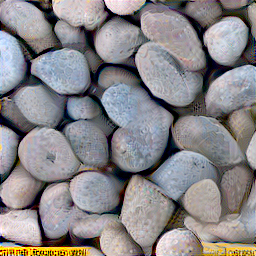
\includegraphics[width=\textwidth]{images/01-pixels_vs_stats-pixels_target.jpg}
            \caption*{\(y_1\)}
            \label{fig:intro_pixels_vs_stats-pixels_target}
        \end{subfigure}
        \hfill
        \begin{subfigure}{0.2\textwidth}
            \centering
            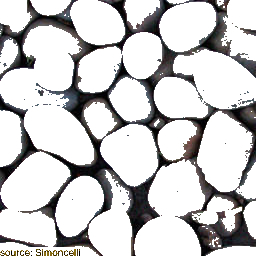
\includegraphics[width=\textwidth]{images/01-pixels_vs_stats-bg.jpg}
            \caption*{Scene}
            \label{fig:intro_pixels_vs_stats-pixels_bg}
        \end{subfigure}
        \hfill
        \begin{subfigure}{0.2\textwidth}
            \centering
            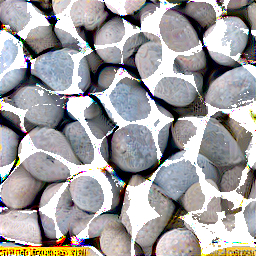
\includegraphics[width=\textwidth]{images/01-pixels_vs_stats-pixels_opt.jpg}
            \caption*{\(p_1\)}
            \label{fig:intro_pixels_vs_stats-pixels_opt}
        \end{subfigure}
        \hfill
        \begin{subfigure}{0.2\textwidth}
            \centering
            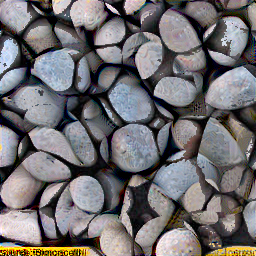
\includegraphics[width=\textwidth]{images/01-pixels_vs_stats-pixels_proj.jpg}
            \caption*{\(x(p_1)\)}
            \label{fig:intro_pixels_vs_stats-pixels_proj}
        \end{subfigure}
        
        \begin{subfigure}{0.2\textwidth}
            \centering
            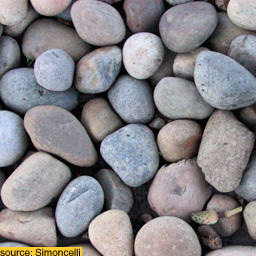
\includegraphics[width=\textwidth]{images/01-pixels_vs_stats-stats_target.jpg}
            \caption*{\(y_2\)}
            \label{fig:intro_pixels_vs_stats-stats_target}
        \end{subfigure}
        \hfill
        \begin{subfigure}{0.2\textwidth}
            \centering
            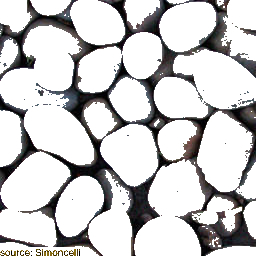
\includegraphics[width=\textwidth]{images/01-pixels_vs_stats-bg.jpg}
            \caption*{Scene}
            \label{fig:intro_pixels_vs_stats-stats_bg}
        \end{subfigure}
        \hfill
        \begin{subfigure}{0.2\textwidth}
            \centering
            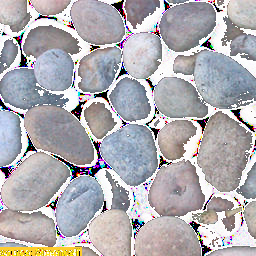
\includegraphics[width=\textwidth]{images/01-pixels_vs_stats-stats_opt.jpg}
            \caption*{\(p_2\)}
            \label{fig:intro_pixels_vs_stats-stats_opt}
        \end{subfigure}
        \hfill
        \begin{subfigure}{0.2\textwidth}
            \centering
            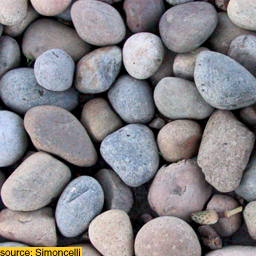
\includegraphics[width=\textwidth]{images/01-pixels_vs_stats-stats_proj.jpg}
            \caption*{\(x(p_2)\)}
            \label{fig:intro_pixels_vs_stats-stats_proj}
        \end{subfigure}
    \end{subfigure}
    \caption{This illustration shows two examples of projection mapping. In the top row, image \(y_1\) cannot be mapped onto the given scene because of the dark areas that reflect little light. Even when projector brightness is set to maximum in those areas (white pixels in image \(p_1\)) according to eq. \ref{eq:projection_mapping-per_pixel}, the final appearance \(x(p_1)\) does not match the desired appearance \(y_1\). In other terms, \(y_1\) fulfills eq. \ref{eq:projection_mapping-hard_image}. On the other hand, image \(y_2\) can be mapped without issues because its bright areas are well aligned with highly reflective parts of the scene and vice versa. Texture source: \citet{Gatys2015}, modified}
    \label{fig:intro_pixels_vs_stats}
\end{figure}

In this thesis, we reformulate the projection mapping recipe in eq. \ref{eq:projection_mapping-per_pixel} to overcome this limitation. We then present a technique that uses our new recipe to achieve results that have not been achieved before when projecting a particular class of images -- textures.

\section{Key Idea}
\label{section:intro-key_idea}

In this section we outline the main idea of overcoming hardware limitations of projectors as introduced above and explain why we focus on projecting textures. For clarity, we provide only a high-level explanation and leave more detailed formal treatment of textures and other concepts for section \ref{section:background-texture_synthesis}.

Textures (e.g. a pebble beach) have the interesting property that when their features (e.g. individual pebbles) are shuffled, the texture still looks the same. We say that a texture has multiple \textit{realizations}. Figure \ref{fig:intro_pixels_vs_stats} shows an example of two different realizations (\(y_1\) and \(y_2\)) of the same texture. Moreover, in that particular example, one can be mapped, while the other cannot. This is the key idea of our thesis and here is how we apply it in projection mapping:

\begin{itemize}
    \item We assume a texture whose given realization is difficult to map onto a given scene because of projector limitations
    \item Out of all possible realizations of that texture we find the one that is the easiest to map
    \item We find the appropriate compensated projection image for it
\end{itemize}

We use this idea to modify the projection mapping recipe from eq. \ref{eq:projection_mapping-per_pixel}. Instead of trying to match each corresponding pair of pixels of camera image \(x(p)\) and desired appearance \(y\), we try to force \(x(p)\) and \(y\) to be realizations of the same texture:

\begin{equation}
    \label{eq:projection_mapping-statistics}
    \min_p || f(x(p)) - f(y) ||
\end{equation}

where \(f\) represents a set of summary statistics of an image and has the property that \(f(y_1) \sim f(y_2)\) \textit{iff} images \(y_1\) and \(y_2\) are realizations of the same texture. Note that eq. \ref{eq:projection_mapping-statistics} is strictly more general than eq. \ref{eq:projection_mapping-per_pixel} because \(x(p) = y\) implies \(f(x(p)) = f(y)\), but the reverse implication does not hold.

Figure \ref{fig:intro_pixels_vs_stats} serves as an example of how our recipe could be applied. With given desired appearance \(y_1\), scene (as shown in the figure) and projector, \(p_2\) is a solution to eq. \ref{eq:projection_mapping-statistics}. \(f(x(p_2)) \sim f(y_1)\), but \(x(p_2) \neq y_1\). On the other hand, if the desired appearance was \(y_2\), then \(p_2\) would solve both eq. \ref{eq:projection_mapping-per_pixel} and \ref{eq:projection_mapping-statistics}.

A suitable set of statistics \(f\), an algorithm that can optimize according to eq. \ref{eq:projection_mapping-statistics} and the ability to integrate both into a projector-camera system are the three main components of our method for projection mapping of textures which we present in this thesis.

\section{Contributions}
\label{section:intro-contributions}

This thesis focuses on a problem of projection mapping exemplified in the upper row of figure \ref{fig:intro_pixels_vs_stats} where a projector is not able to match the desired appearance of a texture due to hardware limitations. Our contributions to solving this problem are the following:

\begin{itemize}
    \item We reformulate the recipe of projection mapping as described in eq. \ref{eq:projection_mapping-per_pixel} to accommodate it better to the projection mapping of textures. Our proposed recipe is described in section \ref{section:intro-key_idea}
    \item Our recipe needs a suitable set of summary statistics (referred to as \(f\) in eq. \ref{eq:projection_mapping-statistics}) which would capture the essence of a texture and be the same across all realizations of the same texture. This problem has been well studied in the field of \textit{texture synthesis} (state-of-the-art report by \citet{Raad2018}) which we introduce and integrate a modified version of neural-based summary statistics by \citet{Gatys2015} into our method
    \item We simulate a projector-camera system in software and implement our method on top of the simulation. It consists of an optimization algorithm that solves eq. \ref{eq:projection_mapping-statistics} in PyTorch
    \item We guide the reader through three experiments whose aim is to evaluate the three key components of our proposed method. Here are the components and a brief summary of the related experiments:
    \begin{enumerate}
        \item \textbf{Algorithm to solve eq. \ref{eq:projection_mapping-statistics}.} In a toy example, our method is able to generate a texture that is both part of a given texture class (as defined by a given texture model) and adapted to fit a given scene well
        \item \textbf{Texture statistics \(f\).} We evaluate a few known texture models in the context of our method and conclude that in certain challenging conditions our method outperforms current pixel-based projection mapping methods as expected. Example shown in fig. \ref{fig:intro_result_teaser}
        \item \textbf{Projector-camera system integration.} Most projection mapping examples in this section project onto flat textured walls. However, our method also works well in virtual 3D scenes with complex geometry and global illumination effects. This constitutes the first step towards real-world application
    \end{enumerate}
\end{itemize}

\begin{figure}[ht]
    \centering    
    \begin{subfigure}{\textwidth}
        \centering
        \begin{subfigure}{0.3\textwidth}
            \centering
            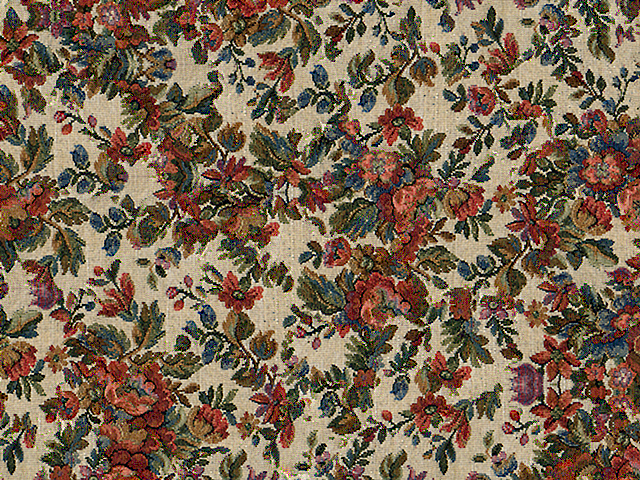
\includegraphics[width=\textwidth]{images/01-results_teaser-target.jpg}
            \caption{Desired appearance}
            \label{fig:intro_results_teaser_target}
        \end{subfigure}
        \hfill
        \begin{subfigure}{0.3\textwidth}
            \centering
            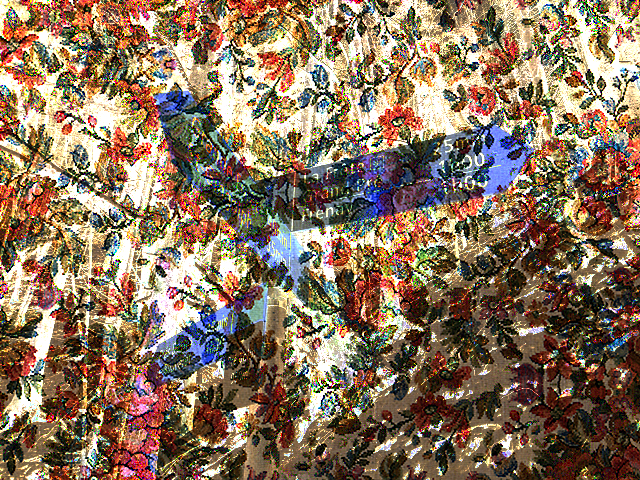
\includegraphics[width=\textwidth]{images/01-results_teaser-pixels_opt.jpg}
            \caption{PB compensation}
            \label{fig:intro_results_teaser_pixels_opt}
        \end{subfigure}
        \hfill
        \begin{subfigure}{0.3\textwidth}
            \centering
            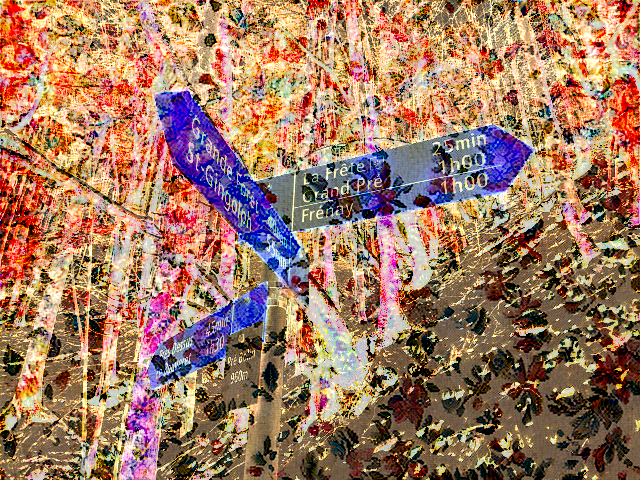
\includegraphics[width=\textwidth]{images/01-results_teaser-stats_opt.jpg}
            \caption{Our compensation}
            \label{fig:intro_results_teaser_stats_opt}
        \end{subfigure}
        
        \begin{subfigure}{0.3\textwidth}
            \centering
            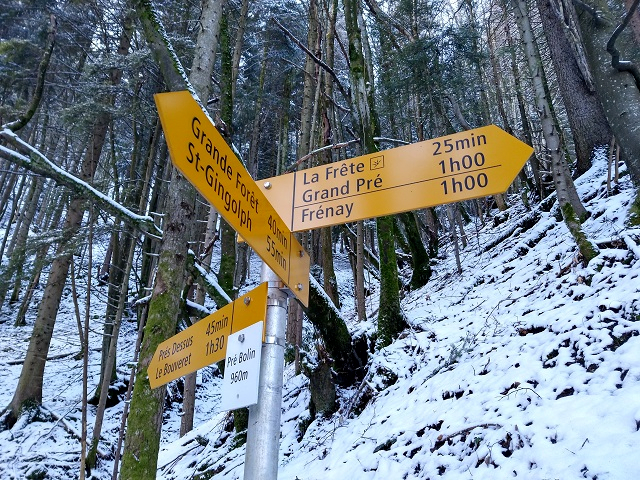
\includegraphics[width=\textwidth]{images/01-results_teaser-bg.jpg}
            \caption{Scene}
            \label{fig:intro_results_teaser_bg}
        \end{subfigure}
        \hfill
        \begin{subfigure}{0.3\textwidth}
            \centering
            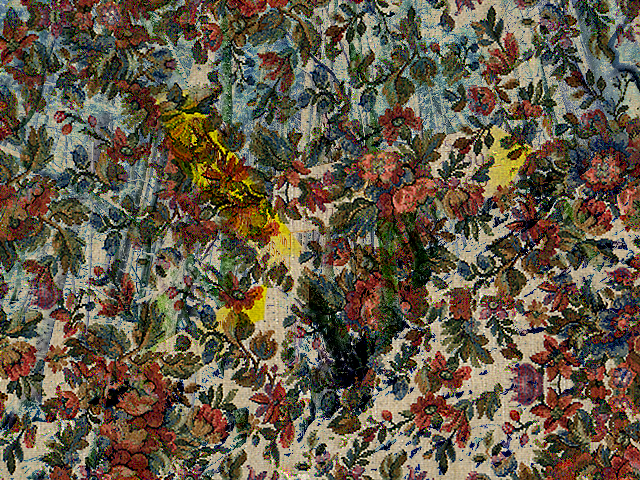
\includegraphics[width=\textwidth]{images/01-results_teaser-pixels_proj.jpg}
            \caption{PB final appearance}
            \label{fig:intro_results_teaser_pixels_proj}
        \end{subfigure}
        \hfill
        \begin{subfigure}{0.3\textwidth}
            \centering
            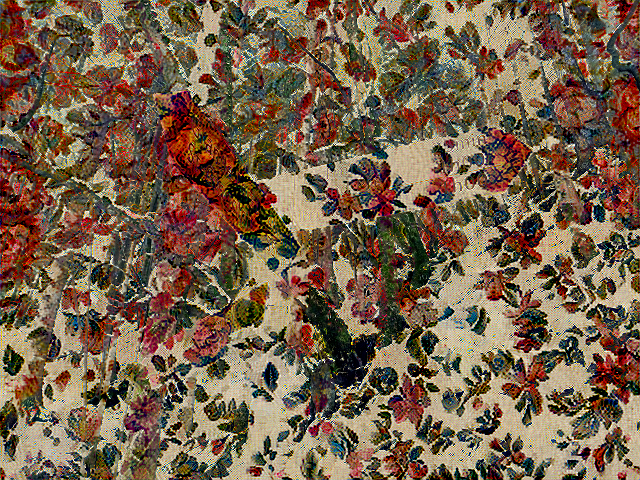
\includegraphics[width=\textwidth]{images/01-results_teaser-stats_proj.jpg}
            \caption{Our final appearance}
            \label{fig:intro_results_teaser_stats_proj}
        \end{subfigure}
    \end{subfigure}
    \caption{Result from one of our experiments. Our scene is a photograph with dark areas and saturated yellow areas which our desired appearance cannot be mapped onto using a conventional pixel-based approach (middle column). Our method (right column) finds a different realization of the input texture which aligns red and beige elements with the yellow sign and dark elements with the forested part of the background. This results in easier mapping (overall lower pixel brightness in fig. \ref{fig:intro_results_teaser_stats_opt} compared to fig. \ref{fig:intro_results_teaser_pixels_opt}) and more faithful reproduction of the desired appearance. Texture source: \citet{Pixar128}, modified}
    \label{fig:intro_result_teaser}
\end{figure}

\section{Thesis Structure}
\label{section:intro-thesis_structure}

This thesis is organized as follows. In chapter \ref{chapter:background}, we provide an overview of the state of the art in projection mapping and texture synthesis and explain in detail the methods which we build on later on. In chapter \ref{chapter:methods}, we describe our method and its implementation. In chapter \ref{chapter:results}, we present the experiments and analyze their results. Lastly, in chapter \ref{chapter:conclusions} we conclude the thesis and discuss future work, particularly with respect to application in real-world projector-camera systems.
